%; whizzy paragraph -pdf xpdf -latex ./whizzypdfptex.sh
%; whizzy-paragraph "^\\\\begin{frame}"
% latex beamer presentation.
% platex, latex-beamer でコンパイルすることを想定。 

%     Tokyo Debian Meeting resources
%     Copyright (C) 2009 Junichi Uekawa
%     Copyright (C) 2009 Nobuhiro Iwamatsu

%     This program is free software; you can redistribute it and/or modify
%     it under the terms of the GNU General Public License as published by
%     the Free Software Foundation; either version 2 of the License, or
%     (at your option) any later version.

%     This program is distributed in the hope that it will be useful,
%     but WITHOUT ANY WARRANTY; without even the implied warranty of
%     MERCHANTABILITY or FITNESS FOR A PARTICULAR PURPOSE.  See the
%     GNU General Public License for more details.

%     You should have received a copy of the GNU General Public License
%     along with this program; if not, write to the Free Software
%     Foundation, Inc., 51 Franklin St, Fifth Floor, Boston, MA  02110-1301 USA

\documentclass[cjk,dvipdfmx,12pt]{beamer}
\usetheme{Tokyo}
\usepackage{monthlypresentation}

%  preview (shell-command (concat "evince " (replace-regexp-in-string "tex$" "pdf"(buffer-file-name)) "&"))
%  presentation (shell-command (concat "xpdf -fullscreen " (replace-regexp-in-string "tex$" "pdf"(buffer-file-name)) "&"))
%  presentation (shell-command (concat "evince " (replace-regexp-in-string "tex$" "pdf"(buffer-file-name)) "&"))

%http://www.naney.org/diki/dk/hyperref.html
%日本語EUC系環境の時
\AtBeginDvi{\special{pdf:tounicode EUC-UCS2}}
%シフトJIS系環境の時
%\AtBeginDvi{\special{pdf:tounicode 90ms-RKSJ-UCS2}}

\title{東京エリア Debian 勉強会}
\subtitle{資料}
\author{岩松 信洋 iwamatsu@debian.or.jp\\IRC nick: iwamatsu}
\date{2009年9月16日}
\logo{
\includegraphics[width=8cm]{image200607/openlogo-light.eps}}

\begin{document}

\frame{\titlepage{}}

\emtext{設営準備にご協力ください}

\section{}
\begin{frame}
 \frametitle{Agenda}
\begin{minipage}[t]{0.45\hsize}
  \begin{itemize}
  \item 注意事項
	\begin{itemize}
	 \item 特になし
	\end{itemize}
  \item 最近あったDebian関連のイベント報告
	\begin{itemize}
	 \item 前回の勉強会
	\end{itemize}
 \end{itemize}
\end{minipage} 
\begin{minipage}[t]{0.45\hsize}
 \begin{itemize}
  \item GPG キーサインパーティの説明
  \item GPG キーサインパーティを楽に済ませるためのツール caff の紹介
  \item キーサインパーティ
 \end{itemize}
\end{minipage}
\end{frame}

\section{最近}

\begin{frame}
 \frametitle{2009年8月}
\begin{minipage}[t]{0.45\hsize}
  \begin{itemize}
  \item 注意事項
	\begin{itemize}
	 \item 飲食禁止
	\end{itemize}
  \item 最近あったDebian関連のイベント報告
	\begin{itemize}
	 \item 前回の勉強会
	\end{itemize}
 \end{itemize}
\end{minipage} 
\begin{minipage}[t]{0.45\hsize}
 \begin{itemize}
  \item Debian JP Project 会長就任の挨拶
  \item Debconf9 報告会
  \item 夏休みの宿題
 \end{itemize}
\end{minipage}
\end{frame}

\begin{frame}{Hack Cafe}

毎週水曜日、週に一回東京のどっかのカフェでハック。\\
\url{http://twitter.com/debian_hackcafe}\\
関西でも始めたようです。\\
(今日はHack Cafeも兼ねています。)
\end{frame}

\begin{frame}{2009年計画}

{\scriptsize
 \begin{enumerate}
  \item 新年の企画 (アンサンブル荻窪開催)
  \item OSC Tokyo
  \item VAIO P インストール記録、
	カーネル読書会 ディストリビューション大集合(小林さん)(東京大学?)
  \item Git Handson (岩松)(あんさんぶる荻窪?)
  \item 家Debianサーバ vs 職場のネットワーク(千代田区都立図書館?\footnote{\url{http://www.library.chiyoda.tokyo.jp/}})
  \item DDTSS 
  \item スペインにて開催
  \item Debconf報告会
  \item Asterisk (東京大学?)、udev + HAL
  \item OSC Fall? (10月30・31日)
  \item 3D graphics 開発 
  \item Debian サーバ+VMware + 各種OS、
	他の仮想化ツール(vserver etc.)、
	忘年会
 \end{enumerate}
}
\end{frame}
\emtext{GPG キーサインパーティの説明}

\begin{frame}{なぜキーサインするのか?}

\end{frame}

\begin{frame}{なぜキーサインするのか?}
\begin{center}
\Huge リア充
\end{center}
\end{frame}

\begin{frame}{なぜキーサインするのか?}
\begin{itemize}
\item PGP/GnuPGは認証局がないので、自分が相手を信頼するしかない。
\item キーサインパーティを行って、PGP/GnuPGの公開鍵をソーシャルな情報とともに交換し、信頼の輪(web of
 trust)を広げる。
\end{itemize}
\end{frame}

\begin{frame}
\begin{center}
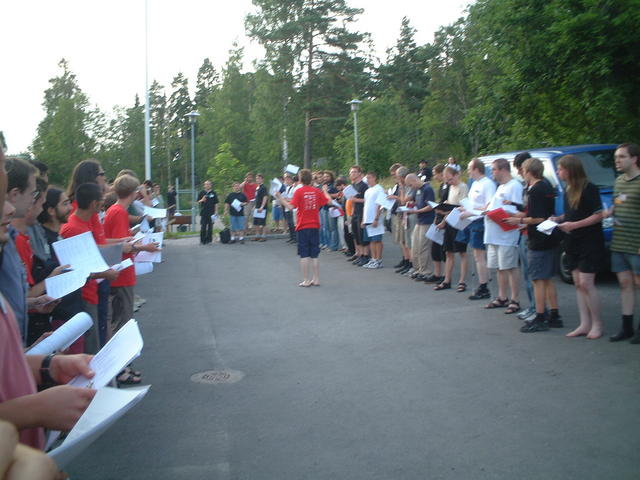
\includegraphics[width=1\hsize]{image200909/ksp00.jpg}

\end{center}
\end{frame}

\begin{frame}
\begin{center}

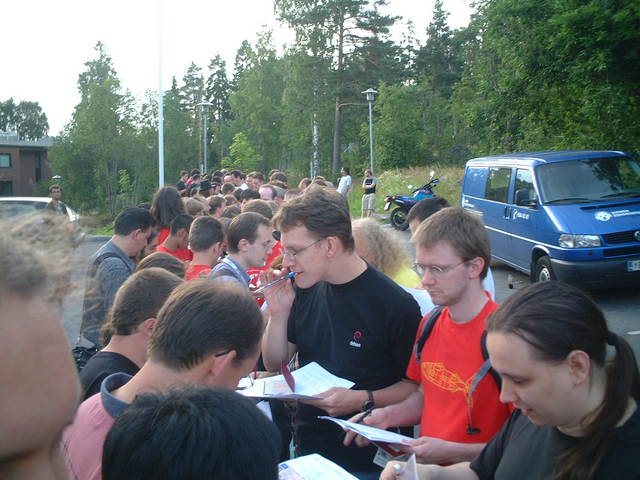
\includegraphics[width=1\hsize]{image200909/ksp01.jpg}
\end{center}
\end{frame}

\begin{frame}
\begin{center}
\Huge 使いどころ
\end{center}
\end{frame}

\begin{frame}{フリーソフトウェア開発者の場合}
\begin{itemize}
\item アカウント作成時のチェックに使ったり。(インターネット上での存在を
      示す。)
\item ソフトウェアのリリース時に使ったり。
\item Debian ではパッケージへの署名、投票などに使う。
\end{itemize}
\end{frame}

\begin{frame}[containsverbatim]{ユーザの場合は?}
\begin{itemize}
\item メールへの署名/暗号化に利用。
\item Debian 開発者になるための通過儀礼。
\end{itemize}
\end{frame}

\begin{frame}[containsverbatim]{ユーザの場合は?}
Linux カーネルのリリースチェック。ちゃんと Linus がタグを打っているのか!
\begin{commandline}
$ git tag -v v2.6.31
object 74fca6a42863ffacaf7ba6f1936a9f228950f657
type commit
tag v2.6.31
tagger Linus Torvalds <torvalds@linux-foundation.org> 1252534447 -0700

Linux 2.6.31
gpg: 2009年09月10日 07時14分11秒 JSTにDSA鍵ID 76E21CBBで施された署名
gpg: 署名を検査できません: 公開鍵が見つかりません
error: could not verify the tag 'v2.6.31'
\end{commandline}
\end{frame}

\begin{frame}[containsverbatim]{ユーザの場合は?}
身近なところでは、改竄のチェックにつかう。
Debian の場合は secure-apt で使われている。
\begin{commandline}
# apt-get update
.....
W: GPG error: http://cdn.debian.or.jp testing Release: The following
 signatures couldn't be verified because the public key is not
 available: NO_PUBKEY 9AA38DCD55BE302B
\end{commandline}
\end{frame}

\begin{frame}[containsverbatim]{ユーザの場合は?}
\begin{commandline}
# gpg --keyserver wwwkeys.eu.pgp.net --recv-keys 9AA38DCD55BE302B
# gpg --armor --export 9AA38DCD55BE302B | apt-key add -
# apt-get update
.....
Fetched 2B in 1s (1B/s)
Reading package lists... Done
\end{commandline}
エラーがでなくなった!これで大丈夫です!(って書いてあるWebサイト多
 いよね。)
\end{frame}

\begin{frame}[containsverbatim]{ユーザの場合は?}
じゃなくて、ちゃんと鍵と信頼度をチェックしましょう。\\
鍵のチェックをするには、Web Of Trust に入らないとできない。
\end{frame}

\begin{frame}[containsverbatim]{チェックする簡単な方法}
9AA38DCD55BE302B の鍵に署名している人は以下のとおり。
\begin{commandline}
pub  4096R/55BE302B 2009-01-27            
uid Debian Archive Automatic Signing Key (5.0/lenny) <ftpmaster@debian.org>
sig  sig3  55BE302B 2009-01-27 _____ 2012-12-31 [selfsig]
sig  sig   7E7B8AC9 2009-01-27 _____ __________ Joerg Jaspert <joerg@debian.org>
sig  sig   D0EC0723 2009-01-27 _____ __________ Mark Hymers <mhy@debian.org>
sig  sig   BE9BF8DA 2009-01-27 _____ __________ Mike O'Connor (stew) <stew@vireo.org>
sig  sig   30B94B5C 2009-05-24 _____ __________ ******** (imacat) <imacat@mail.imacat.idv.tw>
\end{commandline}
\end{frame}
\begin{frame}[containsverbatim]{鍵のチェック}
\begin{commandline}
$ gpg --keyserver pgp.mit.edu --recv-keys 55BE302B
$ gpg --list-sig 55BE302B
pub   4096R/55BE302B 2009-01-27 [満了: 2012-12-31]
uid                  Debian Archive Automatic Signing Key (5.0/lenny)
<ftpmaster@debian.org>
sig          7E7B8AC9 2009-01-27  [ユーザーIDが見つかりません]
sig          D0EC0723 2009-01-27  [ユーザーIDが見つかりません]
sig          BE9BF8DA 2009-01-27  [ユーザーIDが見つかりません]
sig          30B94B5C 2009-05-24  [ユーザーIDが見つかりません]
sig 3        55BE302B 2009-01-27  Debian Archive Automatic Signing Key (5.0/lenny) <ftpmaster@debian.org>
\end{commandline}
だれともサインしていないようです。
\end{frame}


\begin{frame}[containsverbatim]{trust path finder}
しかしWeb of Trust なので、信頼のパスが使える。\\
trust path finder を使うと、信頼のパスが分かる。\\
\url{http://pgp.cs.uu.nl/mk_path.cgi}
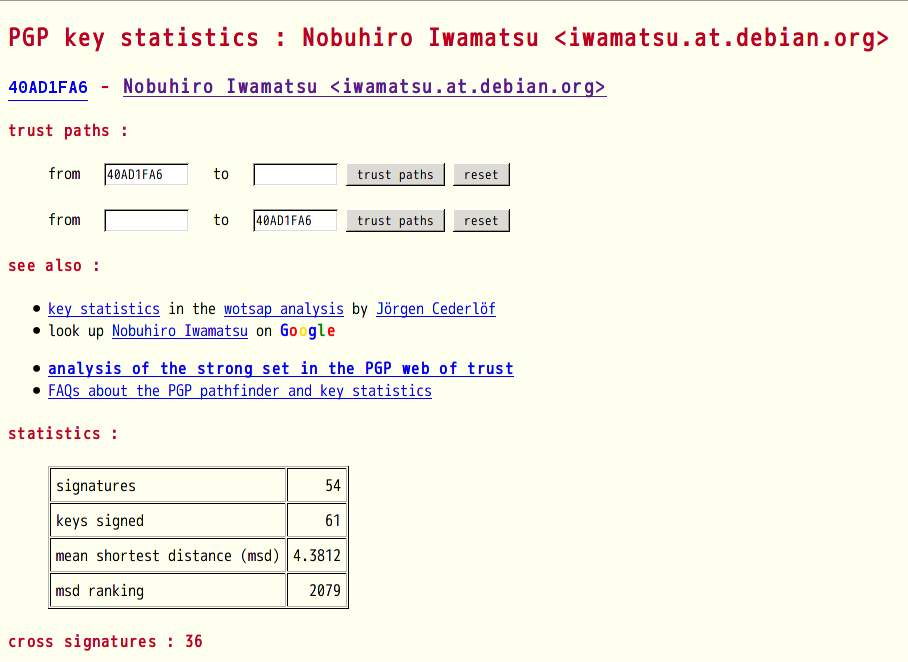
\includegraphics[width=1\hsize]{image200909/trust-path.png}
\end{frame}


\begin{frame}[containsverbatim]{Joergと岩松の trust path}
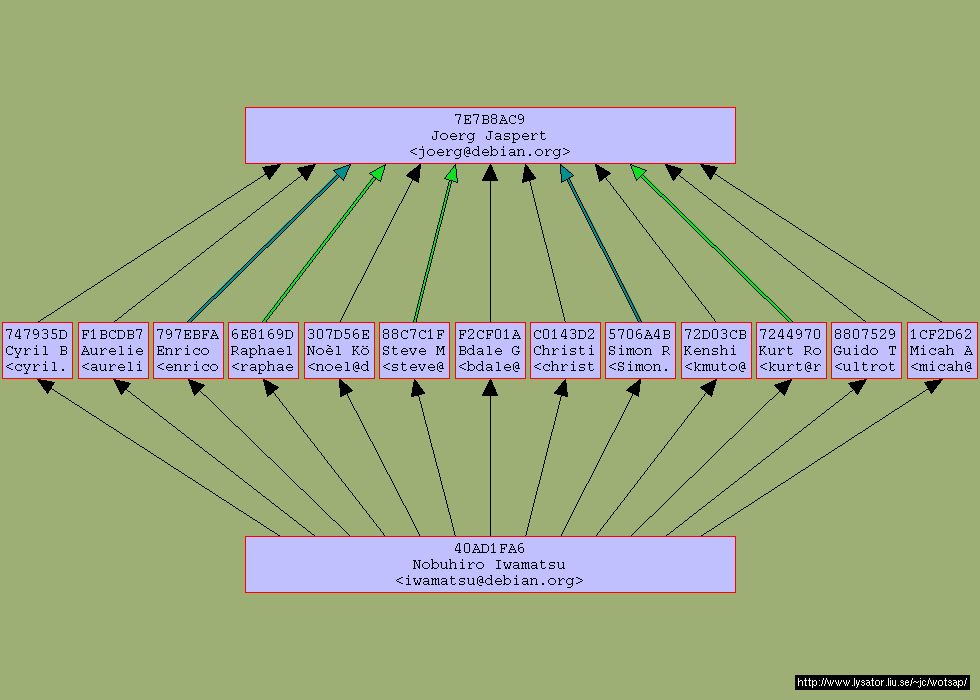
\includegraphics[width=1\hsize]{image200909/0x40AD1FA6-0x7E7B8AC9.png}
他の人を介して、Web of Trust がつながっていることが分かる。
知り合いの知り合いがサインしているようだ。ちょっとは信用できるかな?とか。
\end{frame}

\emtext{GPG キーサインパーティを楽に済ませるためのツール caff の紹介}

\begin{frame}{相手に鍵を送るまでがキーサインパーティです}
相手に鍵を送るまでがキーサインパーティです。
ちゃんと相手に署名した鍵を送りましょう。
\end{frame}

\begin{frame}{キーサインの流れ}
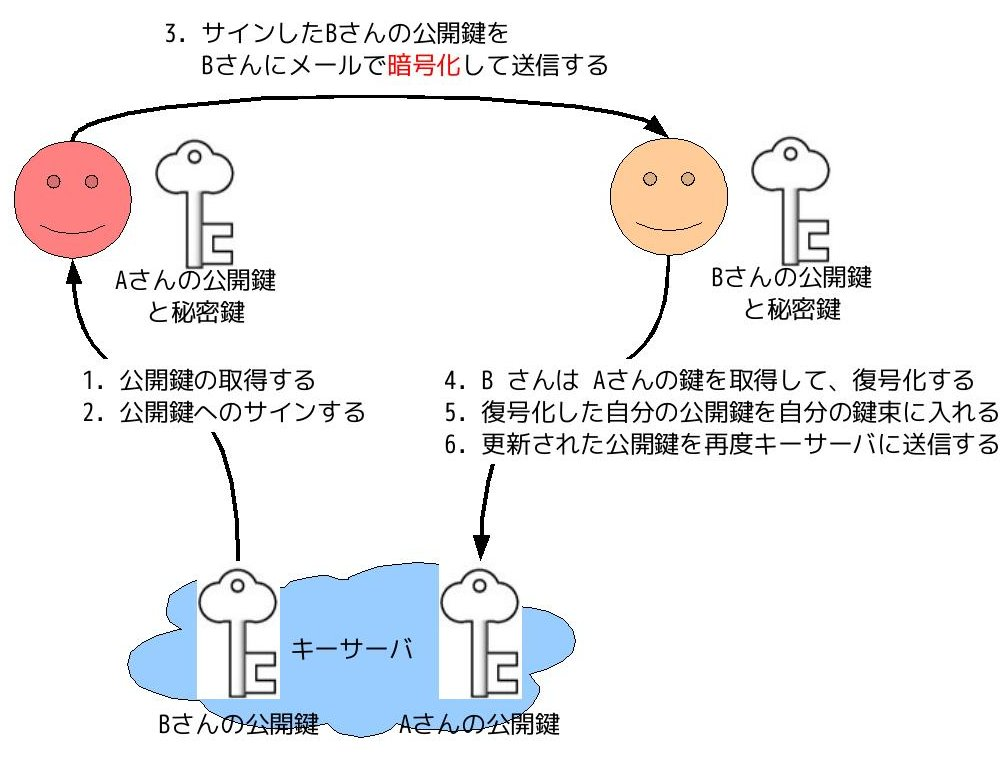
\includegraphics[width=1\hsize]{image200909/gpg-key.jpg}
\end{frame}

\begin{frame}[containsverbatim]{gpg のコマンドでやった場合}
\begin{commandline}
$ gpg --keyserver pgp.mit.edu --recv-key 40AD1FA6
$ gpg --fingerprint 40AD1FA6
$ gpg --edit-key 40AD1FA6
$ gpg --sign-key 40AD1FA6
$ gpg --check-sig 40AD1FA6                   
$ gpg --export -a 40AD1FA6 > iwamatsu.gpgkey   
$ iwamatsu.gpgkey を 相手にメールに 署名+暗号化して送信
\end{commandline}
\end{frame}

\begin{frame}
\begin{center}
\Huge 数人ならいいけど、100人とかやってられん!
\end{center}

\end{frame}

\begin{frame}
\begin{center}
\Huge そこでcaffの登場
\end{center}

\end{frame}

\begin{frame}[containsverbatim]{インストール}
caff は signing-party パッケージで提供されている。
\begin{commandline}
$ sudo apt-get install signing-party
\end{commandline}
\end{frame}

\begin{frame}[containsverbatim]{初期化}
caff を使うための初期化を行う。
caff を一回実行すると、初期ファイルを作成してくれる。
\begin{commandline} 
$ caff
.......
#
#Regards,
#{$owner}
#EOM

Please edit /home/hoge/.caffrc and run caff again.
\end{commandline}
\end{frame}

\begin{frame}[containsverbatim]{caffの設定}
\~{}/.caffrc にある 設定ファイルを修正する。
\begin{commandline}
$ cat ~/.caffrc

$CONFIG{'owner'} = 'Nobuhiro Iwamatsu';
$CONFIG{'email'} = 'iwamatsu@debian.org';

$CONFIG{'keyid'} = [ qw{4121C7433170EBE9 32247FBB40AD1FA6} ]

# Additionally encrypt messages for these keyids
$CONFIG{'also-encrypt-to'} = [ qw{4121C7433170EBE9 32247FBB40AD1FA6} ]

# Mail template to use for the encrypted part
$CONFIG{'mail-template'} = << 'EOM'\maketitle#Hi,

please find attached the user id{(scalar @uids >= 2 ? 's' : '')}
{foreach $uid (@uids) {
    $OUT .= ``\t''.$uid.''\n'';
};}of your key {$key} signed by me.
......

\end{commandline}
\end{frame}

\begin{frame}[containsverbatim]{caffの設定}          

caff のデフォルトの設定では、cert-digest-algo が SHA1 になっているので、
 \footnote{http://bugs.debian.org/cgi-bin/bugreport.cgi?bug=527944} SHA512に
 設定する。
\begin{commandline}
$ mkdir -p ~/.caff/gnupghome
$ chmod 700 ~/.caff/gnupghome
$ cat >> ~/.caff/gnupghome/gpg.conf
cert-digest-algo SHA512
personal-digest-preferences SHA512
EOF
\end{commandline}
\end{frame}

\begin{frame}[containsverbatim]{ローカルSMTPの設定}
ローカル(作業するマシン)のSMTPを設定しておく必要がある。
\end{frame}

\begin{frame}[containsverbatim]{caffを使った署名}
署名するID をキーサーバから取得し、指定した自分のIDで署名してくれる。
そして、署名した鍵を暗号化して送信してくれる。

\begin{commandline}
$ caff -u 自分のID 署名するID .......
\end{commandline}

\end{frame}

\begin{frame}[containsverbatim]{署名完了後}
署名後のデータは \~{}/.gnupg/pubring.gpg ではなく、{\bf \~{}/.caff/gnupghome/pubring.gpg} に格納
 される。この鍵束を \~{}/gnupg/pubring.gpg に 取り込む。
\begin{commandline}
$ gpg --import ~/.caff/gnupghome/pubring.gpg
\end{commandline}

取り込んだら、自分の鍵をキーサーバに送信。
\begin{commandline}
$ gpg --keyserver pgp.nic.ad.jp --send-keys 自分のID
$ gpg --keyserver pgp.mit.edu --send-keys 自分のID
\end{commandline}
\end{frame}


\emtext{キーサインパーティ}

\begin{frame}{キーサインパーティ}
\Huge みんなで sha256ハッシュをチェックしましょう。
\end{frame}

\begin{frame}{キーサインパーティ}
\begin{center}
\Huge 7be4 db5f 8cef 8aa5 \\
\Huge 70d8 f3ac b564 8d7d \\
\Huge ef81 739e 6298 1b5b \\
\Huge 004a a646 44ab 00a7 \\
\end{center}
\end{frame}

\begin{frame}{キーサインパーティ}
\begin{center}
\Huge Enjoy GPG Key Signing Party!
\end{center}
\end{frame}

\end{document}

;;; Local Variables: ***
;;; outline-regexp: "\\([ 	]*\\\\\\(documentstyle\\|documentclass\\|emtext\\|section\\|begin{frame}\\)\\*?[ 	]*[[{]\\|[]+\\)" ***
;;; End: ***
